\documentclass[12pt,a4paper]{article}

\usepackage{fontspec}
\setmainfont{Sarabun}[
  Path = {C:/Users/qwert/AppData/Local/Microsoft/Windows/Fonts/} ,
  Extension = .ttf ,
  UprightFont = *-Regular ,
  BoldFont = *-Bold ,
  ItalicFont = *-Italic ,
  BoldItalicFont = *-BoldItalic ]
\usepackage{graphicx}
\usepackage{amsmath}
\usepackage{amssymb}
\usepackage{geometry}
\usepackage{booktabs}
\usepackage{array}
\usepackage{hyperref}
\usepackage{fancyhdr}
\usepackage{xcolor}
\usepackage{float}
\usepackage{caption}
\usepackage{tcolorbox}
\tcbuselibrary{breakable}

\geometry{margin=1in}
\emergencystretch=1.5em
\setlength{\headheight}{14.5pt}
\linespread{1.25}
\pagestyle{fancy}
\fancyhf{}
\rhead{\thepage}
\lhead{ความรู้: Small-Signal Stability}

\hypersetup{colorlinks=true, linkcolor=blue, urlcolor=blue}

\newcommand{\dwr}{\Delta\omega_r}
\newcommand{\ddel}{\Delta\delta}
\newcommand{\dpsifd}{\Delta\psi_{fd}}

% กล่องสรุปประเด็นสำคัญ
\newtcolorbox{keybox}[1]{colback=blue!4, colframe=blue!50!black,
  fonttitle=\bfseries, title=#1, breakable}

\title{\textbf{สรุปความรู้: การวิเคราะห์เสถียรภาพสัญญาณเล็ก\\
ของระบบเครื่องกำเนิดไฟฟ้าเดี่ยวต่อบัสอนันต์ (SMIB)}\\
\large เอกสารประกอบความเข้าใจ อ้างอิงตำรา Kundur บทที่ 12}
\author{เอกสารความรู้ภาษาไทย คู่กับรายงานภาษาอังกฤษ \texttt{report\_smib}}
\date{31 พฤษภาคม 2569}

\raggedbottom

\begin{document}

\maketitle
\thispagestyle{empty}

\begin{abstract}
\noindent
เอกสารนี้สรุปความรู้พื้นฐานเรื่อง \textbf{เสถียรภาพสัญญาณเล็ก}
(small-signal stability) ของระบบไฟฟ้ากำลัง โดยใช้แบบจำลอง
\textbf{เครื่องกำเนิดไฟฟ้าเดี่ยวต่อบัสอนันต์} (Single-Machine Infinite-Bus,
SMIB) ตามตำรา Kundur บทที่ 12 จุดประสงค์คือให้ผู้อ่านเข้าใจ
\emph{ที่มาของสมการ ความหมายเชิงฟิสิกส์ และผลลัพธ์} ก่อนที่จะไปอ่าน
รายงานภาษาอังกฤษและโค้ด MATLAB ที่พัฒนาขึ้น เนื้อหาเรียงจากแบบจำลอง
ที่ง่ายที่สุด (classical) ไปจนถึงแบบที่มีตัวควบคุมแรงดัน (AVR) และ
ตัวรักษาเสถียรภาพ (PSS)
\end{abstract}

\tableofcontents
\newpage

\section{เสถียรภาพสัญญาณเล็กคืออะไร}

\textbf{เสถียรภาพสัญญาณเล็ก} คือความสามารถของระบบไฟฟ้าในการรักษาการทำงาน
แบบซิงโครนัส (synchronism) เมื่อถูกรบกวนด้วยสัญญาณรบกวนขนาดเล็ก เช่น
การเปลี่ยนแปลงโหลดเล็กน้อย เนื่องจากการรบกวนมีขนาดเล็กมาก เราจึงสามารถ
\textbf{ลิเนียไรซ์ (linearize)} สมการของระบบรอบ ๆ จุดทำงาน (operating point)
ได้ แล้วใช้ \textbf{ค่าลักษณะเฉพาะ (eigenvalues)} ของเมทริกซ์สถานะ (state
matrix) เป็นตัวบอกเสถียรภาพ

\begin{keybox}{หลักการชี้ขาดเสถียรภาพ}
ระบบจะ \textbf{เสถียร} ก็ต่อเมื่อค่าลักษณะเฉพาะ \emph{ทุกตัว} มีส่วนจริง
เป็นลบ ($\sigma < 0$)
\begin{itemize}
  \item ส่วนจริง $\sigma$ เป็นลบ $\rightarrow$ การสั่นลดลง (เสถียร)
  \item ส่วนจริง $\sigma$ เป็นบวก $\rightarrow$ การสั่นโตขึ้น (ไม่เสถียร)
  \item ส่วนจินตภาพ $\omega$ $\rightarrow$ ความถี่ของการสั่น
\end{itemize}
\end{keybox}

\subsection{แรงบิดสองชนิดที่กระทำต่อโรเตอร์}

หัวใจของเรื่องนี้คือแรงบิดไฟฟ้า (electrical torque) ที่กระทำต่อโรเตอร์
ของเครื่องกำเนิด แยกได้เป็นสององค์ประกอบ:

\begin{itemize}
  \item \textbf{แรงบิดซิงโครไนซ์ (synchronizing torque)} --- อยู่ในเฟส
        เดียวกับการเบี่ยงเบนมุมโรเตอร์ $\ddel$ ถ้าไม่พอ ระบบจะเสียเสถียรภาพ
        แบบ \emph{ลู่ออกทางเดียว} (ไม่สั่น)
  \item \textbf{แรงบิดหน่วง (damping torque)} --- อยู่ในเฟสเดียวกับการ
        เบี่ยงเบนความเร็ว $\dwr$ ถ้าไม่พอ ระบบจะเสียเสถียรภาพแบบ
        \emph{สั่นโตขึ้นเรื่อย ๆ}
\end{itemize}

โหมดการสั่นที่เราสนใจที่สุดเรียกว่า \textbf{โหมดสวิง (swing mode)} หรือ
โหมดไฟฟ้า-กล (electromechanical mode) ซึ่งเป็นการแกว่งของโรเตอร์เทียบกับ
ระบบ มีความถี่ประมาณ $0.1$--$2$ เฮิรตซ์

\section{ระบบ SMIB และสัญลักษณ์}

ระบบ SMIB คือเครื่องกำเนิดไฟฟ้าหนึ่งเครื่องต่อผ่านหม้อแปลงและสายส่งไปยัง
\textbf{บัสอนันต์} (infinite bus --- แรงดันและความถี่คงที่ เปรียบเหมือน
กริดขนาดใหญ่มาก) ตัวแปรและพารามิเตอร์หลัก:

\begin{table}[H]
\centering
\caption{สัญลักษณ์ที่ใช้}
\begin{tabular}{@{}cl@{}}
\toprule
สัญลักษณ์ & ความหมาย \\
\midrule
$H$        & ค่าคงที่ความเฉื่อย (inertia constant) \\
$K_D$      & สัมประสิทธิ์แรงบิดหน่วง \\
$K_S$      & สัมประสิทธิ์แรงบิดซิงโครไนซ์ \\
$\omega_0$ & ความเร็วฐาน $= 2\pi f_0$ (rad/s) \\
$\ddel$    & การเบี่ยงเบนมุมโรเตอร์ \\
$\dwr$     & การเบี่ยงเบนความเร็วโรเตอร์ (pu) \\
$\dpsifd$  & การเบี่ยงเบนเส้นแรงแม่เหล็กขดสนาม \\
$X_d'$     & รีแอกแตนซ์ชั่วครู่แกน $d$ \\
$E_B$      & แรงดันบัสอนันต์ \\
$K_A, T_R$ & อัตราขยายและค่าคงที่เวลาของตัวควบคุมแรงดัน (AVR) \\
\bottomrule
\end{tabular}
\end{table}

\section{แบบจำลอง 4 ระดับ}

เราสร้างแบบจำลอง 4 ระดับ ไล่จากง่ายไปซับซ้อน แต่ละระดับเพิ่มฟิสิกส์
เข้ามาทีละชั้น

\subsection{แบบ Classical (2 สถานะ)}

มองเครื่องกำเนิดเป็นแรงดันคงที่ $E'$ หลังรีแอกแตนซ์ $X_d'$ สมการการแกว่ง
(swing equation) แบบลิเนียไรซ์ (Kundur สมการ 12.78):

\begin{equation}
\frac{d}{dt}
\begin{bmatrix} \dwr \\ \ddel \end{bmatrix}
=
\begin{bmatrix}
-\dfrac{K_D}{2H} & -\dfrac{K_S}{2H} \\[2ex]
\omega_0 & 0
\end{bmatrix}
\begin{bmatrix} \dwr \\ \ddel \end{bmatrix}
+
\begin{bmatrix} \dfrac{1}{2H} \\[2ex] 0 \end{bmatrix}
\Delta T_m
\end{equation}

โดยสัมประสิทธิ์แรงบิดซิงโครไนซ์หาได้จากความสัมพันธ์กำลัง-มุม:

\begin{equation}
K_S = \frac{E' E_B}{X_T}\cos\delta_0,
\qquad X_T = X_d' + X_E
\end{equation}

ความถี่ธรรมชาติและอัตราส่วนการหน่วง:

\begin{equation}
\omega_n = \sqrt{\frac{K_S\,\omega_0}{2H}},
\qquad
\zeta = \frac{1}{2}\cdot\frac{K_D}{2H\,\omega_n}
\end{equation}

\begin{keybox}{สิ่งที่แบบ A สอนเรา}
ความถี่ของโหมดสวิงถูกกำหนดโดย $K_S$ และ $H$ ส่วนการหน่วงมาจาก $K_D$
โดยตรง --- ถ้า $K_D = 0$ จะได้การสั่นแบบไม่หน่วง (ค่าลักษณะเฉพาะอยู่บน
แกนจินตภาพพอดี) ในตัวอย่าง 12.2 ได้ $f_n = 1.02$ เฮิรตซ์
\end{keybox}

\subsection{เพิ่มพลวัตขดสนาม (3 สถานะ)}

เพิ่มเส้นแรงแม่เหล็กขดสนาม $\dpsifd$ เป็นสถานะที่สาม เพื่อจับผลของ
\textbf{ปฏิกิริยาอาร์เมเจอร์} (armature reaction) ที่ทำให้สนามแม่เหล็ก
ลดลงช้า ๆ เมทริกซ์สถานะ (Kundur สมการ 12.116):

\begin{equation}
A_B =
\begin{bmatrix}
-\dfrac{K_D}{2H} & -\dfrac{K_1}{2H} & -\dfrac{K_2}{2H} \\[2ex]
\omega_0 & 0 & 0 \\[1ex]
0 & a_{32} & a_{33}
\end{bmatrix}
\end{equation}

โดย $a_{32} = -K_3 K_4/T_3$, $a_{33} = -1/T_3$ ค่าคงที่ $K_1$ ถึง $K_4$
คือ \textbf{ค่าคงที่ Heffron--Phillips} ซึ่งในงานนี้เรา
\textbf{คำนวณเองจากพารามิเตอร์ $d$--$q$ ของเครื่อง} ไม่ได้รับค่าสำเร็จรูป
(ดูหัวข้อ \ref{sec:kderiv})

\subsection{เพิ่มตัวควบคุมแรงดัน AVR (4 สถานะ)}

เพิ่มตัวกระตุ้น (exciter) ชนิดไทริสเตอร์ที่มีอัตราขยาย $K_A$ และตัวแปลง
สัญญาณแรงดัน (transducer) ค่าคงที่เวลา $T_R$ เป็นสถานะที่สี่ $\Delta v_1$
ต้องใช้ค่าคงที่เพิ่มสองตัว: $K_5$ (ผลของมุมโรเตอร์ต่อแรงดันปลายทาง) และ
$K_6$ (ผลของเส้นแรงสนามต่อแรงดันปลายทาง)

การตอบสนองของเส้นแรงสนามต่อการรบกวนมุมโรเตอร์ (Kundur สมการ 12.144):

\begin{equation}
\frac{\dpsifd}{\ddel}(s) =
\frac{-K_3\bigl[K_4(1+sT_R) + K_5 K_A\bigr]}
     {(1+sT_3)(1+sT_R) + K_3 K_6 K_A}
\end{equation}

\begin{keybox}{ข้อแลกเปลี่ยนสำคัญของ AVR (เมื่อ $K_5 < 0$)}
เมื่อเพิ่มอัตราขยาย $K_A$:
\begin{itemize}
  \item แรงบิดซิงโครไนซ์ $K_S$ \textbf{เพิ่มขึ้น} (ดี)
  \item แรงบิดหน่วง $K_D$ \textbf{ลดลงจนติดลบ} (อันตราย!)
\end{itemize}
ในตาราง 12.1 ที่ $K_A = 200$ ได้ $K_D = -12.27$ ทำให้โหมดสวิง
\textbf{ไม่เสถียร} ($+0.504 \pm j7.23$)
\end{keybox}

\subsection{เพิ่มตัวรักษาเสถียรภาพ PSS (6 สถานะ)}

\textbf{ตัวรักษาเสถียรภาพระบบไฟฟ้า} (Power System Stabilizer, PSS) แก้ปัญหา
แรงบิดหน่วงติดลบ โดยป้อนสัญญาณเสริมจาก $\dwr$ ผ่านวงจรชดเชย (Kundur
สมการ 12.151):

\begin{equation}
G_{PSS}(s) = K_{STAB}\,
\underbrace{\frac{sT_w}{1+sT_w}}_{\text{washout}}\,
\underbrace{\frac{1+sT_1}{1+sT_2}}_{\text{lead-lag}}
\end{equation}

\begin{itemize}
  \item \textbf{Washout} ($sT_w/(1+sT_w)$): กรองสัญญาณความถี่ต่ำ/ค่าคงที่
        ออก เพื่อไม่ให้ PSS ไปยุ่งกับการทำงานปกติของ AVR
  \item \textbf{Lead-lag} ($(1+sT_1)/(1+sT_2)$): เพิ่มมุมเฟสนำ (phase lead)
        เพื่อชดเชยมุมเฟสล้าหลังของระบบกระตุ้น
\end{itemize}

ผลคือแปลงแรงบิดหน่วงติดลบกลับเป็นบวก ทำให้โหมดสวิงกลับมาเสถียร

\section{การคำนวณค่าคงที่ $K$ จากพารามิเตอร์ $d$--$q$}
\label{sec:kderiv}

จุดเด่นของงานนี้คือเรา \textbf{ไม่รับค่า $K$ สำเร็จรูป} แต่คำนวณจาก
พารามิเตอร์เครื่องโดยตรง ตามขั้นตอนตัวอย่าง 12.3:

\begin{enumerate}
  \item \textbf{ความอิ่มตัว (saturation):} เส้นแรงรวม $\psi_{at}$ ที่จุดทำงาน
        กำหนดค่าตัวประกอบความอิ่มตัว เมื่อเกินค่าเริ่ม $\psi_{T1}$ ใช้
        $K_{sd}^{incr} = 1/(1 + B_{sat}\psi_I)$
  \item \textbf{จุดทำงาน:} หามุมภายในตรง ๆ
        $\delta_0 = \operatorname{atan2}(E_{Bd0}, E_{Bq0})$ แล้วจึงหากระแสแกน
        $d$--$q$, กระแสสนาม $i_{fd0}$ และแรงดันสนาม $E_{fd0}=L_{adu}i_{fd0}$
  \item \textbf{สัมประสิทธิ์การคู่ควบ:} $m_1, n_1, m_2, n_2$ (สมการ
        12.106--108) --- \emph{จุดที่ต้องระวัง:} $m_2, n_2$ ใช้ $L_{ads}$
        แบบ \emph{incremental} (ไม่ใช่ค่าขนาน $L_{ads}'$)
  \item \textbf{ค่าคงที่ $K$:} ประกอบเป็น $K_1, K_2$; ส่วน $K_4$ มาจาก
        $a_{32} = -(\omega_0 R_{fd}/L_{adu})K_4$ (สังเกตว่าเป็น $L_{adu}$
        ไม่ใช่ $L_{fd}$); และ $T_3 = -1/a_{33}$
\end{enumerate}

\begin{keybox}{บทเรียนจากการ debug จริง}
ระหว่างพัฒนา พบจุดพลาด 2 จุดที่ทำให้ค่าไม่ตรงตำรา จนแก้ได้:
(1) สูตรมุม $\delta_0$ ต้องใช้ \texttt{atan2} ตรง ๆ ไม่ต้องลบมุมภายใน;
(2) $m_2, n_2$ ต้องใช้ $L_{ads}$ แบบ incremental และ $K_4$ ใช้ $L_{adu}$
หลังแก้แล้วค่าทุกตัวตรงตำราภายใน $1\%$
\end{keybox}

\section{ผลลัพธ์และการตรวจสอบ}

โค้ด \texttt{run\_smib\_example.m} รันบน MATLAB R2026a เทียบกับค่าอ้างอิง
จากตำรา ทำการตรวจสอบ 26 รายการ \textbf{ผ่านทั้งหมด} แต่ละหัวข้อด้านล่าง
แสดง \emph{โจทย์ (ข้อมูลที่ให้)} $\rightarrow$ \emph{วิธีทำ} $\rightarrow$
\emph{ผลเทียบตำรา}

\subsection{ตัวอย่าง 12.2 --- แบบ Classical}

\begin{keybox}{โจทย์ (Kundur Ex.\ 12.2)}
เครื่องกำเนิด 2220 MVA, 24 kV, 60 Hz, $H=3.5$, $X_d'=0.30$ pu จ่ายกำลัง
$P=0.9$, $Q=0.3$ pu ที่แรงดันปลายทาง $E_t=1.0\angle 36^\circ$ pu
รีแอกแตนซ์ภายนอกถึงบัสอนันต์ $X_E=0.65$ pu, แรงดันบัสอนันต์
$E_B=0.995\angle 0^\circ$ pu \\
\textbf{หา:} จุดทำงาน, $K_S$, และค่าลักษณะเฉพาะที่ $K_D=0, 10, -10$
\end{keybox}

\textbf{วิธีทำ:}
\begin{enumerate}
  \item กระแสปลายทางจาก $S=E_t I_t^{*}$:
        $I_t = 0.9487\angle 17.57^\circ = 0.9045 + j0.2863$ pu
  \item แรงดันภายในหลังรีแอกแตนซ์ชั่วครู่:
        $E' = E_t + jX_d' I_t = 1.1229\angle 49.91^\circ$ pu
  \item มุมโรเตอร์: $\delta_0 = \angle E' - \angle E_B = 49.91^\circ$
  \item $X_T = X_d' + X_E = 0.95$ pu
  \item $K_S = \dfrac{|E'||E_B|}{X_T}\cos\delta_0 =
        \dfrac{1.1229\times0.995}{0.95}\cos 49.91^\circ = 0.7574$
  \item $\omega_n = \sqrt{K_S\omega_0/(2H)} = 6.387$ rad/s $= 1.0165$ Hz
\end{enumerate}

\begin{table}[H]
\centering
\caption{ตัวอย่าง 12.2 --- ผลเทียบตำรา}
\begin{tabular}{@{}lrr@{}}
\toprule
ปริมาณ & คำนวณได้ & ค่าตำรา \\
\midrule
$\delta_0$ (องศา)      & 49.91 & 49.92 \\
$|E'|$ (pu)            & 1.123 & 1.123 \\
$K_S$                  & 0.7574 & 0.757 \\
$f_n$ (Hz)             & 1.0165 & 1.0165 \\
$\lambda$ ($K_D{=}0$)  & $\pm j6.39$ & $\pm j6.39$ \\
$\lambda$ ($K_D{=}10$) & $-0.714\pm j6.35$ & $-0.714\pm j6.35$ \\
$\zeta$ ($K_D{=}10$)   & 0.112 & 0.112 \\
\bottomrule
\end{tabular}
\end{table}

\subsection{ตัวอย่าง 12.3 --- พลวัตขดสนาม (ค่า $K$ ที่คำนวณเอง)}

\begin{keybox}{โจทย์ (Kundur Ex.\ 12.3)}
เครื่องและจุดทำงานเดียวกับ 12.2 แต่จำลองพลวัตขดสนาม + ความอิ่มตัว
พารามิเตอร์เครื่อง (pu): $L_{adu}=1.65$, $L_{aqu}=1.60$, $L_l=0.16$,
$R_a=0.003$, $L_{fd}=0.153$, $R_{fd}=0.0006$; ความอิ่มตัว $A_{sat}=0.031$,
$B_{sat}=6.93$, $\psi_{T1}=0.80$ \\
\textbf{หา:} ค่าคงที่ $K_1$--$K_4$, $T_3$ (\emph{คำนวณจากพารามิเตอร์ข้างต้น}),
เมทริกซ์สถานะ และค่าลักษณะเฉพาะ
\end{keybox}

\textbf{วิธีทำ (ตัวเลขกลางทางจริง):}
\begin{enumerate}
  \item \textbf{ความอิ่มตัว:} $\psi_{at}=1.0604 > \psi_{T1}$ ดังนั้น
        $\psi_I=0.1884$ ได้ $K_{sd}=0.8491$, $K_{sd}^{incr}=0.4337$;
        $L_{ads}=1.4011$, $L_{ads}^{incr}=0.7156$
  \item \textbf{มุมภายในและกระแส:} $\delta_i=43.13^\circ$ จากนั้น
        $i_{d0}=0.8342$, $i_{q0}=0.4518$, $e_{d0}=0.6836$, $e_{q0}=0.7299$
  \item \textbf{มุมโรเตอร์และสนาม:} $E_{Bd0}=0.9773$, $E_{Bq0}=0.1876$
        $\rightarrow \delta_0=\operatorname{atan2}(0.9773,0.1876)=79.13^\circ$;
        $i_{fd0}=1.4514 \rightarrow E_{fd0}=2.395$
  \item \textbf{สัมประสิทธิ์คู่ควบ:} $m_1=1.0436$, $n_1=0.1268$,
        $m_2=0.8801$, $n_2=0.00176$
  \item \textbf{ค่า $K$:} $K_1=0.7643$, $K_2=0.8649$, $K_3=0.323$,
        $K_4=1.4187$, $T_3=2.356$ s
\end{enumerate}

เมทริกซ์สถานะและค่าลักษณะเฉพาะที่ได้:
\begin{equation}
A_B =
\begin{bmatrix}
0 & -0.1092 & -0.1236 \\
376.99 & 0 & 0 \\
0 & -0.1945 & -0.4244
\end{bmatrix},
\quad
\lambda =
\begin{cases}
-0.110 \pm j6.411 & \text{(สวิง)} \\
-0.205 & \text{(สนาม)}
\end{cases}
\end{equation}

\begin{table}[H]
\centering
\caption{ตัวอย่าง 12.3 --- ค่าที่คำนวณเทียบตำรา}
\begin{tabular}{@{}lrr@{}}
\toprule
ปริมาณ & คำนวณได้ & ค่าตำรา \\
\midrule
$\delta_0$ (องศา) & 79.13 & 79.13 \\
$E_{fd0}$ (pu)   & 2.395 & 2.395 \\
$m_1$            & 1.0436 & 1.0437 \\
$m_2$            & 0.8801 & 0.8802 \\
$K_1$            & 0.7643 & 0.7643 \\
$K_2$            & 0.8649 & 0.8649 \\
$K_4$            & 1.4187 & 1.4187 \\
$T_3$ (s)        & 2.356 & 2.365 \\
โหมดสวิง         & $-0.110\pm j6.41$ & $-0.110\pm j6.41$ \\
โหมดสนาม         & $-0.205$ & $-0.204$ \\
\bottomrule
\end{tabular}
\end{table}

ตัวประกอบการมีส่วนร่วม (participation) ยืนยันตัวตนของแต่ละโหมด: โหมดสวิง
เป็น $\dwr$ $49\%$ + $\ddel$ $49\%$ มี $\dpsifd$ แค่ $1.7\%$ ส่วนโหมดสนาม
เป็น $\dpsifd$ ถึง $99.8\%$

\subsection{ตาราง 12.1 --- ผลของ AVR}

\begin{keybox}{โจทย์ (Kundur Sec.\ 12.4)}
เครื่องที่มี $K_1=1.591$, $K_2=1.5$, $K_3=0.333$, $K_4=1.8$, $K_5=-0.12$,
$K_6=0.3$, $T_3=1.91$ s, $H=3.0$, ตัวกระตุ้น $T_R=0.02$ s \\
\textbf{หา:} แรงบิดซิงโครไนซ์/หน่วงจากวง field/AVR เปลี่ยนอย่างไรเมื่อเพิ่ม
อัตราขยาย $K_A$
\end{keybox}

\textbf{วิธีทำ:} ใช้สมการ $\dpsifd/\ddel(s)$ (Eq.~12.144) คูณ $K_2$ แล้ว
ประเมินที่ $s=j\omega$ ($\omega\approx10$ rad/s) แยกส่วนจริง = $K_S(\dpsifd)$,
ส่วนจินตภาพ$\times\omega_0/\omega$ = $K_D(\dpsifd)$

\begin{table}[H]
\centering
\caption{ตาราง 12.1 --- องค์ประกอบแรงบิดเทียบ $K_A$ ($\omega=10$ rad/s)}
\begin{tabular}{@{}rrr@{}}
\toprule
$K_A$ & $K_S(\dpsifd)$ & $K_D(\dpsifd)$ \\
\midrule
0   & $-0.0025$ & $+1.770$ \\
15  & $-0.0093$ & $+0.024$ \\
25  & $-0.0098$ & $-1.165$ \\
200 & $+0.2801$ & $-12.271$ \\
\bottomrule
\end{tabular}
\end{table}

เห็นชัดว่า $K_D$ ลดผ่านศูนย์ราว $K_A \approx 15$ แล้วติดลบมากขึ้นเรื่อย ๆ
ที่ $K_A=200$ การวิเคราะห์เต็มได้โหมดสวิงไม่เสถียร $+0.504\pm j7.23$

\subsection{ตัวอย่าง 12.6 --- AVR + PSS ดึงระบบกลับมาเสถียร}

\begin{keybox}{โจทย์ (Kundur Ex.\ 12.6)}
เครื่องตัวอย่าง 12.3 ที่ใส่ AVR อัตราขยายสูง ($K_A=200$) จนโหมดสวิงไม่เสถียร
ออกแบบ PSS: $K_{STAB}=9.5$, washout $T_w=1.4$ s, lead-lag $T_1=0.154$ s,
$T_2=0.033$ s \\
\textbf{แสดงว่า:} PSS ดึงระบบกลับมาเสถียร
\end{keybox}

\textbf{ผล:} ค่าลักษณะเฉพาะครบ 6 ตัวเมื่อมี PSS:
$\lambda=\{-39.10,\ -1.005\pm j6.607,\ -0.739,\ -19.80\pm j12.82\}$
อยู่ครึ่งระนาบซ้ายทั้งหมด โหมดสวิงย้ายจาก $+0.504\pm j7.23$ (AVR อย่างเดียว,
$\zeta=-0.07$) มาเป็น $-1.005\pm j6.607$ ($\zeta=+0.15$)

\begin{table}[H]
\centering
\caption{ผลของ PSS ที่ $K_A=200$}
\begin{tabular}{@{}lrrc@{}}
\toprule
การตั้งค่า & โหมดสวิง & $\zeta$ & เสถียร \\
\midrule
AVR อย่างเดียว & $+0.504\pm j7.23$ & $-0.07$ & ไม่ \\
AVR + PSS      & $-1.005\pm j6.61$ & $+0.15$ & ใช่ \\
\bottomrule
\end{tabular}
\end{table}

\begin{keybox}{ภาพรวมเรื่องราวทั้งหมด}
แบบ A ตั้งความถี่สวิงราว 1 Hz $\rightarrow$ แบบ B ขดสนามเพิ่มการหน่วง
เล็กน้อย $\rightarrow$ แบบ C AVR อัตราขยายสูงทำลายการหน่วงจนไม่เสถียร
$\rightarrow$ แบบ D PSS เติมการหน่วงกลับ ระบบเสถียรอีกครั้ง
\end{keybox}

\section{กราฟประกอบ}

\begin{figure}[H]
\centering
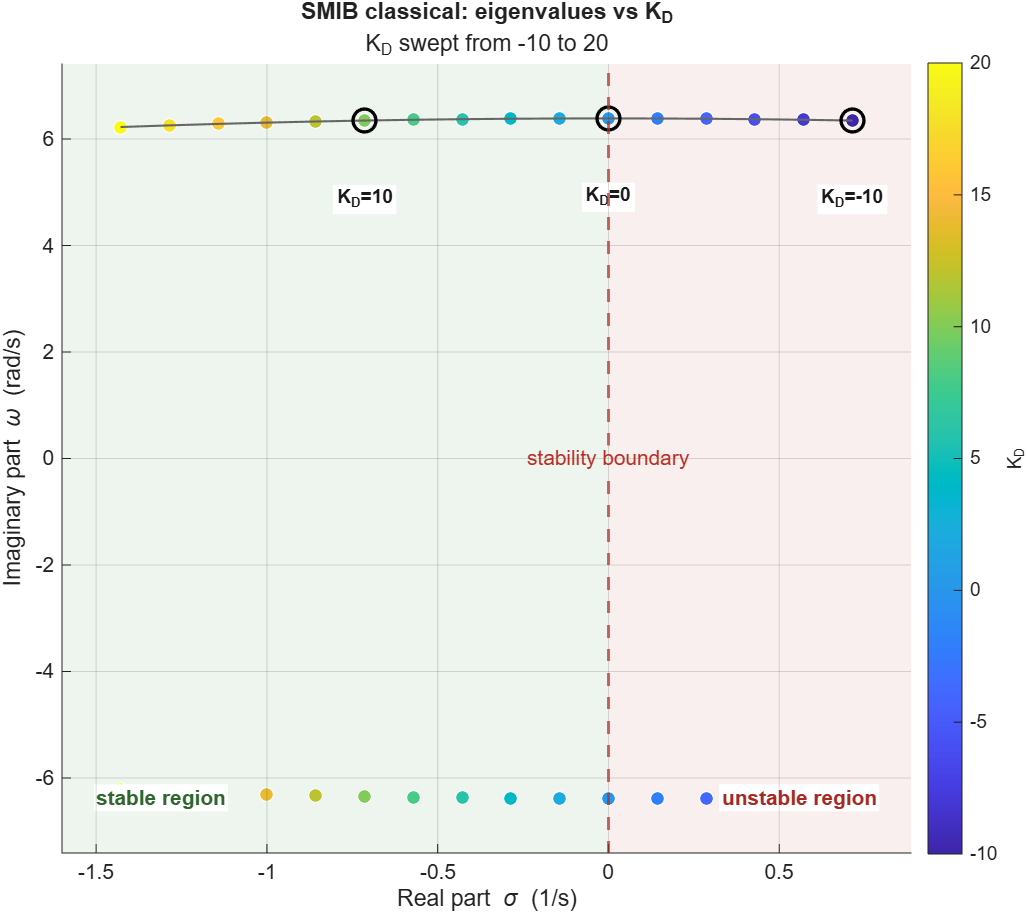
\includegraphics[width=0.85\textwidth]{figures/01_root_locus.png}
\caption{เส้นทางเดินของค่าลักษณะเฉพาะ (root locus) แบบ A เมื่อกวาด $K_D$
จาก $-10$ ถึง $+20$ เส้นข้ามแกนจินตภาพ (ขอบเสถียรภาพ) ที่ $K_D=0$;
$K_D$ ติดลบทำให้ค่าลักษณะเฉพาะเข้าครึ่งระนาบขวา (ไม่เสถียร)}
\end{figure}

\begin{figure}[H]
\centering
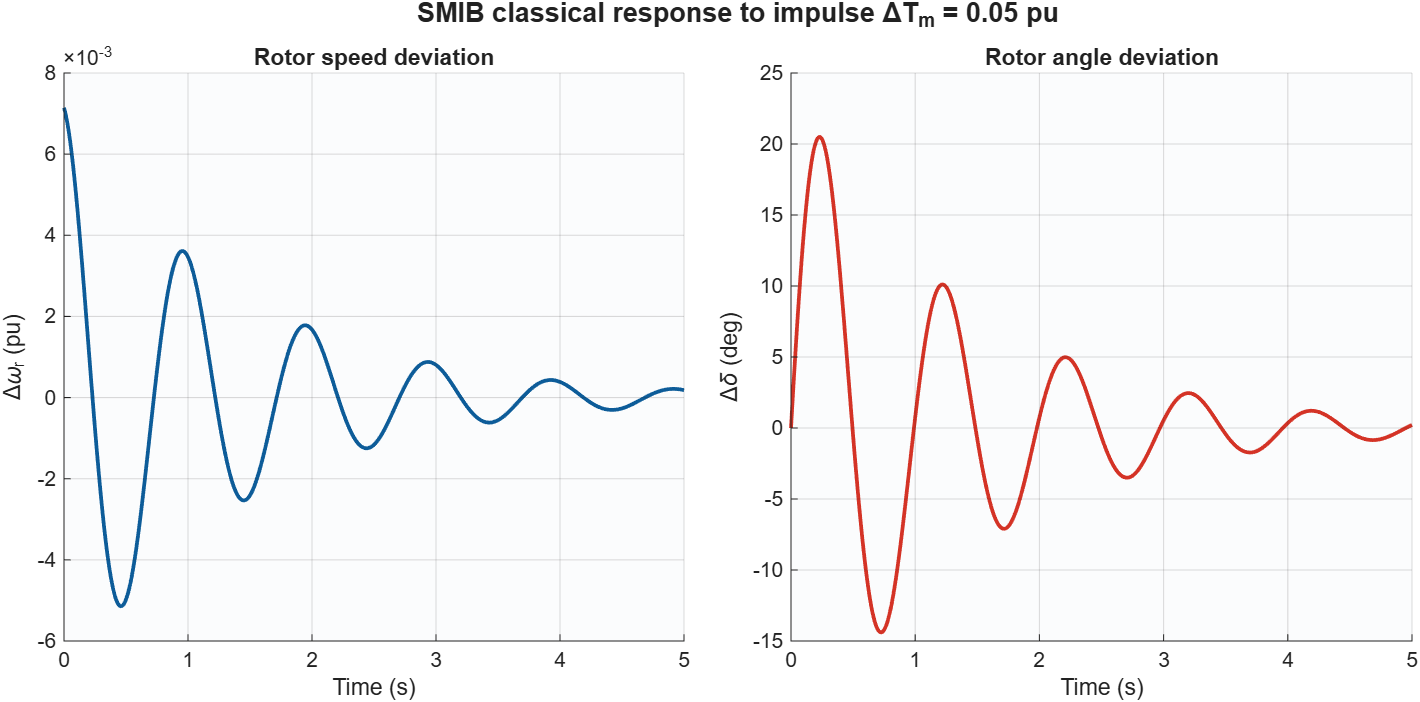
\includegraphics[width=0.85\textwidth]{figures/02_step_response.png}
\caption{การตอบสนองเชิงเวลาของแบบ A ($K_D=10$) ต่อแรงบิดอิมพัลส์เล็กน้อย
การสั่นความถี่ $\sim1$ Hz ลดลงด้วย $\zeta=0.112$}
\end{figure}

\begin{figure}[H]
\centering
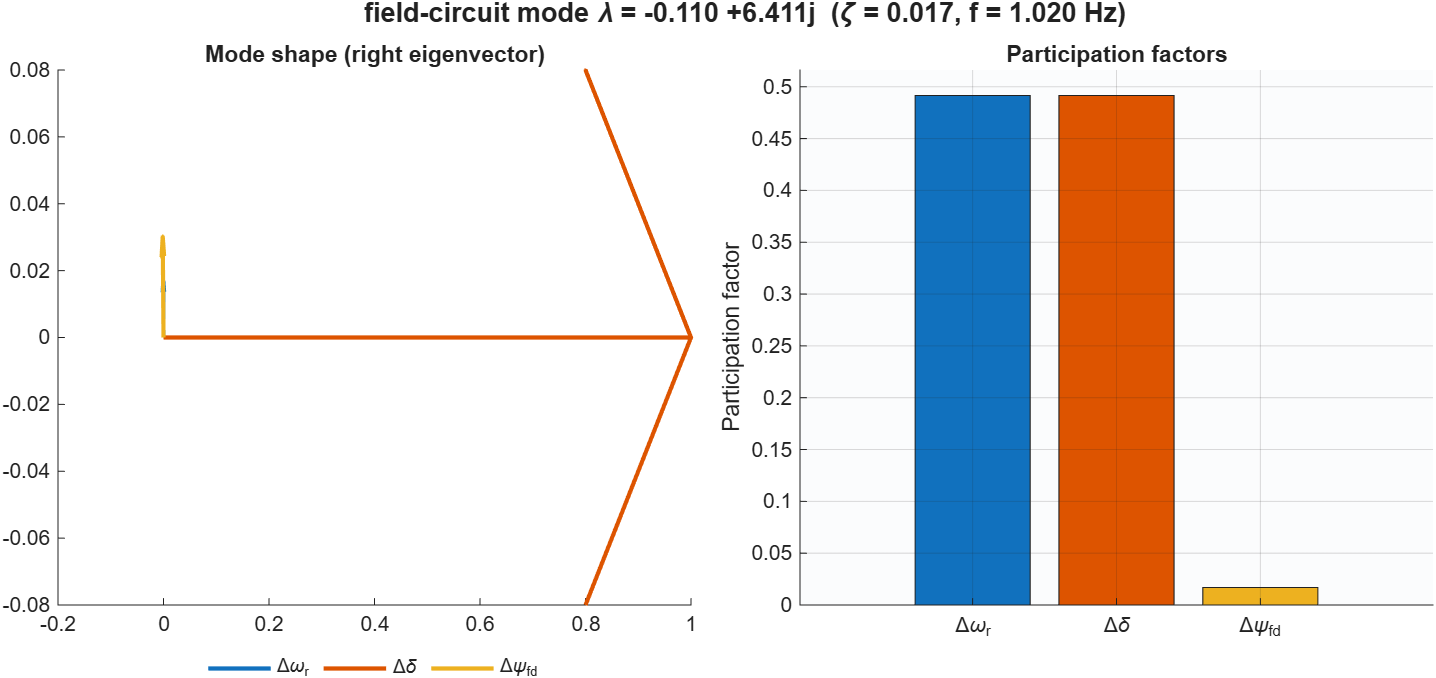
\includegraphics[width=0.85\textwidth]{figures/03_mode_shape.png}
\caption{รูปร่างโหมด (mode shape, ซ้าย) และตัวประกอบการมีส่วนร่วม
(participation factors, ขวา) ของโหมดสวิง แบบ B เห็นว่าสถานะโรเตอร์
$\dwr$ และ $\ddel$ มีบทบาทหลัก ส่วน $\dpsifd$ แทบไม่มีส่วนร่วม}
\end{figure}

\begin{figure}[H]
\centering
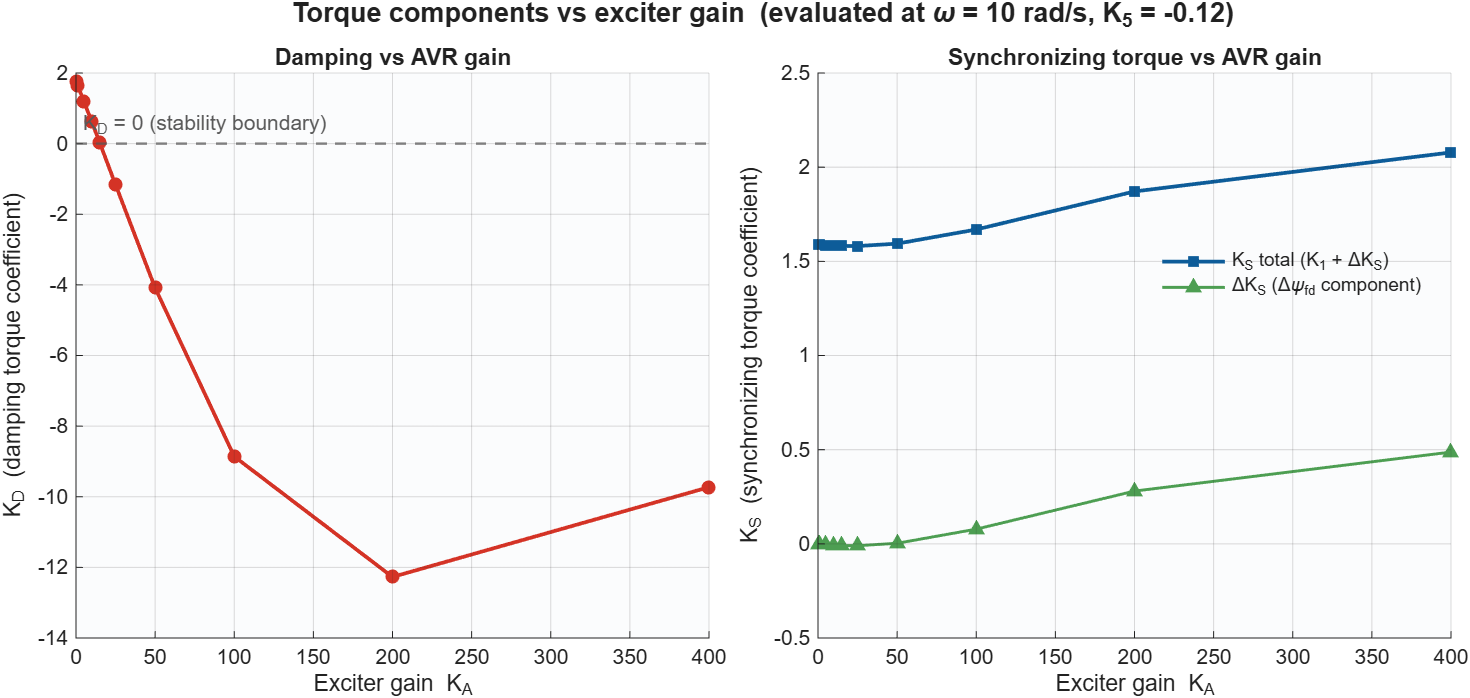
\includegraphics[width=0.85\textwidth]{figures/04_torque_vs_ka.png}
\caption{สัมประสิทธิ์แรงบิดหน่วง (ซ้าย) และซิงโครไนซ์ (ขวา) เทียบอัตราขยาย
AVR เมื่อ $K_5<0$ การเพิ่มอัตราขยายดัน $K_D$ ให้ติดลบ ในขณะที่ $K_S$
เพิ่มขึ้น ตรงตามตาราง 12.1 ของ Kundur}
\end{figure}

\section{สรุป}

เอกสารนี้อธิบายแนวคิดเสถียรภาพสัญญาณเล็กของระบบ SMIB ครบทั้ง 4 แบบจำลอง
ตามตำรา Kundur บทที่ 12 ประเด็นสำคัญที่สุดคือ \textbf{ข้อแลกเปลี่ยนระหว่าง
แรงบิดซิงโครไนซ์กับแรงบิดหน่วง}: AVR อัตราขยายสูงช่วยเรื่องซิงโครไนซ์แต่
ทำลายการหน่วง และ PSS คือคำตอบที่เติมการหน่วงกลับโดยไม่เสียข้อดีของ AVR
ผลการคำนวณทุกแบบจำลองตรงกับค่าอ้างอิงในตำราภายใน $1$--$2\%$ โดยค่าคงที่ $K$
ถูกคำนวณจากพารามิเตอร์ $d$--$q$ ของเครื่องโดยตรง

\vspace{1em}
\noindent\textbf{เอกสารอ้างอิง:} P. Kundur, \textit{Power System Stability
and Control}, McGraw-Hill, 1994, บทที่ 12 (ตัวอย่าง 12.2, 12.3, 12.6;
หัวข้อ 12.4 ตาราง 12.1)

\end{document}
